% Full paper:
% https://github.com/pauldubois98/ESTRO2024/blob/main/full_paper.pdf
\section{Distance Between Doses}
In this section, we aim to establish a robust metric for quantifying the distance between different dose distributions.
Such a distance should provide a numerical comparison that reflects the clinical discrepancies between two dose distributions.
By developing a distance measure that captures these nuances, we can better evaluate and compare treatment plans.

\paragraph{A non-trivial task}
Quantifying the difference between two dose distributions, particularly regarding clinical impact, is inherently challenging.
This complexity arises because not all patient anatomy regions contribute equally to treatment outcomes.
Dose variations in critical structures may significantly influence clinical effects, while similar variations in less critical areas may have negligible impact.
Moreover, the potential for dose compensation (underdosing in one region counterbalancing overdosing in another) further complicates the development of a reliable metric for comparing dose distributions.
This compensatory effect is only sometimes applicable, making establishing a standardized method for assessing dose distribution clinical differences challenging.

\paragraph{Dose Evaluation}
To assess the quality of a dose distribution, dosimetrists primarily focus on DVHs as the key metric.
While they also consider aspects of the three-dimensional (3D) dose distribution, such as inter-structure dose gradients and the presence, number, and location of hot spots, their primary attention is directed towards the analysis of DVHs, which provide a comprehensive overview of dose coverage and sparing of organs at risk.

\subsection{Method}

\paragraph{Naive Doses Comparison}
The most straightforward method for comparing two dose distributions, thus defining a distance metric, is to perform a voxel-by-voxel comparison of the dose values.
However, this approach overlooks the inherent anatomical structure of the human body and the fact that not all voxels have the same clinical significance.
Consequently, even if the voxel-wise distance between two dose distributions is considerable, their overall clinical effects may still be similar.

\paragraph{Pathological example}
We constructed a simplified example, as illustrated in Figure \ref{fig:pathological_example}.
This hypothetical scenario involves a phantom model consisting of a homogeneous water-equivalent material containing a cubic planning target volume (PTV) and a cubic organ-at-risk (OAR).
Although this model lacks anatomical realism, it effectively highlights the limitations of using basic voxel-wise comparisons for dose evaluation.
It emphasizes the need for more sophisticated techniques to capture clinically relevant differences in dose distributions accurately.
\begin{figure}
	\centering
	\begin{subfigure}{0.44\linewidth}
		\includegraphics[width=\linewidth]{dose_distances_figures/example\_3d\_doses.pdf}
		\caption{3D visualization of the two doses on the phantom body.}
		\label{fig:pathological_example-3d_doses}
	\end{subfigure}
	\begin{subfigure}{0.55\linewidth}
		\includegraphics[width=\linewidth]{dose_distances_figures/example\_bixels.pdf}
		\caption{2D view of the bixels activation of the two doses.}
		\label{fig:pathological_example-bixels}
	\end{subfigure}
	\begin{subfigure}{0.75\linewidth}
		\includegraphics[width=\linewidth]{dose_distances_figures/example\_dvh.pdf}
		\caption{Dose-Volume Histograms of the two doses on the phantom body.}
		\label{fig:pathological_example-dvh}
	\end{subfigure}
	\caption{Example of two doses that have the same clinical effect (measured from the DVHs), but very different voxel-wise dose values.}
	\label{fig:pathological_example}
\end{figure}

\subsubsection{Doses Samples}
We assessed the efficacy of our proposed method for comparing radiation doses using the TG-119 Prostate case, a well-established benchmark for evaluating radiation therapy plans \cite{AAPM-TG119}.
The TG-119 dataset includes predefined dose objectives, which we utilized to formulate our cost function.
We performed optimizations with different weight assignments applied to each constraint to generate varying treatment dose distributions for the same patient case under identical constraints.

\subsubsection{Distances Between Doses}
\paragraph{Comparing Doses Voxel-wise}
When two radiation dose distributions are closely aligned, the voxel-wise comparison is an effective measure, as it can be assumed that the global distribution is similar.
This approach allows for a detailed comparison of local dose variations.
Mathematically, given the voxel-wise dose $\textbf{d}$, the distance between two dose distributions, $\textbf{d}^1$ and $\textbf{d}^2$, is defined as the norm of their difference:
$\sum_{v \in \mathcal{V}} \lvert \textbf{d}^1_v - \textbf{d}^2_v \rvert$, where $v$ represents the voxels in the set of interest $\mathcal{V}$, and $\textbf{d}^i_v$ is the dose value at voxel $v$ for dose distribution $\textbf{d}^i$
\footnote{This is often written as $\lvert \textbf{d}_1 - \textbf{d}_2 \rvert$, with the summation over voxels implied.}.
However, voxel-wise distance can become misleading if two regions of equal volume within the same anatomical structure have their dose values swapped.
In such cases, the voxel-wise difference would appear large despite the clinical equivalence of the two doses.
Furthermore, this method is limited to comparing doses within the same patient, as it requires a direct correspondence between the dose voxels in both distributions.

\paragraph{Comparing Dose Volume Histogram Curves}
We propose comparing the Dose Volume Histogram (DVH) curves.
We have one curve for each structure; we define the distances between doses for each structure, and in the end, we sum up all structures to end up with a single scalar distance between two doses.
We can quantify the variation between the two dose distributions in aggregated forms, using the structures.

\subparagraph{Discrete DVH Approximation}
The DVH is obtained after sorting the voxel-wise dose of the structure:
Let $\textbf{d} \left[s\right]$ bet the voxel-wise dose of the structure $s$ (therefore, a list, of length $n\left[s\right]$, the number of voxels that belong to the structure).
Let $\dot{\textbf{d}\left[s\right]}$ be the list above in descending order (i.e. $\dot{\textbf{d}\left[s\right]}_i > \dot{\textbf{d}\left[s\right]}_j$ if $0 < i < j \leq n\left[s\right ]$).
Then, the DVH of $s$ can be approximated by the continuous line composed of the segments linking the following points:
$\left( \dot{\textbf{d}\left[s\right]}_i, i/n\left[s\right] \right) \quad 0 < i \leq n\left[s\right]$.
Since we compute the dose voxel-wise, we may only have an approximation of the DVH.
However, in practice, most structures of interest have more than a hundred voxels, which makes the DVH approximation very precise.

Since we draw one curve per structure of interest, this capture some of the importance of voxel over others.
In fact, when analyzing a dose, doctors look at the dose volume (voxel-wise), but they also take a close look at the DVHs; this is an incentive that DVHs should contain meaningful information.

\subparagraph{Distance Measure}
To measure how different two DVH curves, we can imagine several techniques:
\begin{itemize}
	\item Fréchet distance (treating DVHs as curves in a 2D space)
	\item Hausdorff distance (treating DVHs as 1D manifolds in a 2D space)
	\item Wasserstein distance (treating DVHs as probability distributions)
	\item Kolmogorov-Smirnov test (treating DVHs as probability distributions)
	\item Total variation between curves (treating DVHs as functions)
\end{itemize}
We evaluated all the aforementioned distance metrics and propose to retain only the one that yields the most clinically meaningful results.

\subparagraph{Fréchet Distance}
DVH (Dose-Volume Histogram) curves can be interpreted as lines in R2R2 \footnote{In the case of voxel-wise dose approximations, they are represented as poly-lines in R2R2.}.
In this context, the Fréchet distance is a well-known metric for assessing the similarity between two curves, particularly useful for comparing poly-lines \cite{Efrat2002}.
It measures the minimum distance a particle would travel when simultaneously traversing both curves.
In this study, we apply the Fréchet distance to compare the DVH curves of two radiation dose distributions.

Formally, let $P$ and $Q$ represent the curves being compared, with $\gamma$ denoting a parametrization defined on the interval $\left[0,1\right]$.
The positions of a particle moving along curves $P$ and $Q$ at time $t$ are given by $P(\gamma(t))$ and $Q(\gamma(t))$, respectively.
The Fréchet distance is defined as:
$$d_{\text{Fréchet}}(P,Q) = \inf_{\gamma}{ \max_{t \in \left[ 0,1 \right]} d(P(\gamma(t)), Q(\gamma(t)))}$$

When applied to DVH curves, let $\mathcal{C}_A$ and $\mathcal{C}_B$ denote the discrete DVH curves of two dose distributions.
These curves consist of line segments connecting a series of points $\left\lbrace \mathcal{C}_A(i) = (d_i, v_i), \ 1 \leq i \leq n_A \right\rbrace $ and $\left\lbrace \mathcal{C}_B(j) = (\tilde{d}_j, \tilde{v}_j), \ 1 \leq j \leq n_B \right\rbrace $; where $d_i$ and $\tilde{d}_j$ denote the dose levels\footnote{Derived from $\textbf{d}$ after selecting voxels of the structure of interest, and sorting voxels.}, $v_i$ and $\tilde{v}_j$ represent the corresponding volumes, and $n_A$ and $n_B$ are the number of points forming $\mathcal{C}_A$ and $\mathcal{C}_B$\footnote{Here we are constantly comparing two DVH curves of the same structure on the same patient, so we always have $n_A = n_B$.}.

The Fréchet distance, in this case, is defined as the infimum over all possible traversal times.
Given that the curves are discrete line segments, the Fréchet distance can be expressed as:
$$d_{\text{Fréchet}}(\mathcal{C}_A, \mathcal{C}_B) = \min_{\substack{j: \llbracket 1, n_A \rrbracket \to \llbracket 1, n_B \rrbracket \\ j \nearrow \ (j \text{ increasing})}} \sum_{i=1}^{n_A} dist\left( \mathcal{C}_A(i), \mathcal{C}_B(j(i)) \right)$$
$$\text{where } dist\left( \mathcal{C}_A(i), \mathcal{C}_B(j(i)) \right) = \sqrt{(d_i-\tilde{d}_{j(i)})^2 + (v_i-\tilde{v}_{j(i)})^2}$$

Here, $j$ represents a (discrete) a parametrization, and $dist\left( \mathcal{C}_A(i), \mathcal{C}_B(j(i)) \right)$ is the distance between points $\mathcal{C}_A(i)$ and $\mathcal{C}_B(j(i))$.

One drawback of the Fréchet distance is its computational expense, particularly for structures with a large number of voxels.
To mitigate this, we applied the Ramer–Douglas–Peucker algorithm for curve simplification \cite{PRASAD2012843}.
We employed this algorithm with $\epsilon=0.05$, and after testing on a subset of DVH curves, it was found to accelerate computations by a factor of 3-5, while the calculated Fréchet distance deviated by less than 0.5\%.
This method was therefore used in the results presented below.


\subparagraph{Hausdorff Distance}
The Hausdorff distance is another commonly used metric for measuring the similarity between two curves \cite{Henrikson1999CompletenessAT}.
It is defined as the greatest of the shortest distances between any point on one curve and the closest point on the other.
Formally, let $X$ and $Y$ be two non-empty sets;
the Hausdorff distance between $X$ and $Y$, denoted $d_\text{Hausdorff}(X, Y)$, is given by:
$$d_\text{Hausdorff}(X, Y) = \sup_{x \in X}\inf_{y \in Y} {dist(x, y)}$$
where $dist(x, y)$ represents the distance between points $x$ and $y$ (typically, the Euclidean distance).

In this study, we treat DVH (Dose-Volume Histogram) curves as sets of points in a two-dimensional space $\R^2$, using the Hausdorff distance to quantify their difference.
Using the same notation for the DVH curves $\mathcal{C}_A$ and $\mathcal{C}_B$ as previously defined, the discrete Hausdorff distance is computed as:
$$d_\text{Hausdorff}(\mathcal{C}_A, \mathcal{C}_B) = \max_{i \in \llbracket 1,n_A \rrbracket} \min_{y \in \mathcal{C}_B} {dist(\mathcal{C}_A(i), y)}$$
where $\mathcal{C}_B$ is represented by the set of points
$$\left\lbrace \left( (1-\lambda) \tilde{d}_j + \lambda \tilde{d}_{j+1}, (1-\lambda) \tilde{v}_j + \lambda \tilde{v}_{j+1} \right) \mid \lambda \in \left[ 0,1 \right], j \in \llbracket 1, n_B-1 \rrbracket \right\rbrace.$$
%and $dist$ is the distance between two points as before.

\subparagraph{Wasserstein Distance}
The Wasserstein distance, also known as the Earth Mover’s Distance, is a metric used to quantify the difference between two probability distributions \cite{OLKIN1982257}.
Formally, given two probability distributions $\mu$ and $\nu$ defined on a metric space $X$, the Wasserstein distance, denoted $d_{\text{Wasserstein}}(\mu, \nu)$, represents the infimum cost of transporting the mass of distribution $\mu$ to match distribution $\nu$, where the transportation cost is determined by the distance metric $dist$ on $X$.
It is defined as:
$$d_{\text{Wasserstein}}(P, Q) = \inf_{\gamma \in \Gamma(\mu, \nu)} E_{(x,y) \sim \gamma} \left[ dist(x, y) \right]$$
where $\Gamma(\mu, \nu)$ represents the set of all possible joint distributions $\gamma(x, y)$ with marginals $\mu$ and $\nu$.

In our analysis, we treat DVH (Dose-Volume Histogram) curves as probability distributions and employ the Wasserstein distance to assess their differences.
This metric has the distinct advantage of capturing both local and global variations between the curves, offering a more comprehensive comparison.
However, it can be computationally demanding, particularly when dealing with DVHs of large anatomical structures.

\subparagraph{Kolmogorov-Smirnov Distance}
Another distance metric commonly used to compare dose-volume histogram (DVH) curves is the Kolmogorov-Smirnov (KS) distance \cite{Stephens1974}.
The KS distance measures the maximum vertical separation between two curves and is particularly well-suited for comparing non-parametric distributions, such as DVH curves.

Mathematically, let the two DVH curves be represented by functions $f$ and $g$, mapping dose levels to volume ratios. The KS distance, $d_{KS}$, is then defined as:
$$d_{KS} = \sup_{x \in \R^+} \abs{f(x)-g(x)}.$$

In the case of discrete DVH data, $f$ and $g$ are piecewise linear, continuous functions from $\mathbb{R}^+$ to $[0,1]$, with their values set to zero beyond the maximum dose level.

\subparagraph{Total Variation Distance}
We propose a distance metric that computes the integral of the absolute difference between two DVH (dose-volume histogram) curves.
This metric is straightforward to compute and provides a balanced measure of local and global differences between the curves \cite{Chatterjee2007}.
Additionally, it is computationally efficient and well-suited for analyzing large structures with many voxels.
This approach yielded the most consistent and clinically relevant results among the metrics tested.
As such, we selected this distance measure for our analysis.

Traditionally, the total variation distance is defined as the integral of the absolute difference between two DVH curves.
While the dose domain is theoretically unbounded, the volume domain is bounded between 0 and 100\%.
To avoid integrating over an unbounded dose domain, we opted to reverse the axes, placing dose on the $y$-axis and volume on the $x$-axis and subsequently integrating the absolute difference in dose over the volume range $[0,1]$.

Mathematically, standard DVHs are described by $V: \mathbb{R}^+ \to [0,1]$.
For two DVHs $V(d)$ and $\tilde{V}(d)$, the total variation distance is given by:
$$
d_{\text{TotalVariation}} = \int_{0}^{+\infty} \lvert V(d) - \tilde{V}(d) \rvert \, dd
$$

However, in our approach, we express DVHs with dose as a volume function, denoted $D: [0,1] \to \mathbb{R}^+$.
Thus, for two DVHs $D(v)$ and $\tilde{D}(v)$, the total variation distance becomes:

$$
d_{\text{TotalVariation}} = \int_{0}^{1} \lvert D(v) - \tilde{D}(v) \rvert \, dv
$$

While the theoretical value of the integral remains unchanged, we prefer integrating over the finite volume domain $0,1]$ instead of the unbounded dose domain $\mathbb{R}^+ = [0,+\infty[$.
An illustration highlighting the differences between the classical DVH and the version with swapped $x$- and $y$-axes is presented in Figure \ref{fig:dose_volume_difference}.
The two compared doses were optimized on the TG-119 phantom prostate case, using different weights (1 and 3) for the PTV objective.

\begin{figure}
	\centering
	\includegraphics[width=0.95\textwidth]{dose_distances_figures/dose\_volume\_difference}
	\subfloat[\label{fig:dose_volume_difference-normal} Classical DVH (dose on the $x$-axis)]{\hspace{1\linewidth}}
	
	\centering
	\includegraphics[width=0.95\textwidth]{dose_distances_figures/dose\_volume\_difference-flipped}
	\subfloat[\label{fig:dose_volume_difference-flipped} Flipped axes DVH (volume on the $x$-axis)]{\hspace{1\linewidth}}
	
	\caption{DVHs: Comparison of classical and flipped axes styles.}
	\label{fig:dose_volume_difference}
\end{figure}

As Figure \ref{fig:dose_volume_difference} shows, the difference between DVHs exhibits less noise (fewer fluctuations) when the dose is on the $x$-axis.
This observation suggests a reduction in numerical error, providing additional motivation to place the volume on the $x$-axis.

Computing the total variation distance is computationally efficient, requiring only $\mathcal{O}(n_s)$ operations per structure, where $n_s$ represents the number of voxels in the structure of interest, $s$.
Overall, this method achieves a good balance between capturing local and global differences in DVH curves.

\subsection{Results}
\subsubsection{Dose Distances Comparison}
We optimized each constraint with all weights initially set to 1 but sequentially increased one to 3, 10, and 100.
This process resulted in 18 distinct dose distributions, which were compared using the distance metrics described earlier.
We calculated the pairwise distances for each pair of doses, effectively constructing the adjacency matrix of a fully connected graph, where each optimized dose corresponds to a node.
See Figure \ref{fig:pairwise_distances} for comparing the adjacency matrices.
\begin{figure}
	\centering
	\includegraphics[width=\textwidth]{dose_distances_figures/pairwise\_distances.pdf}
	\caption{Pairwise distances between doses\\(with different distances calculation method)}
	\label{fig:pairwise_distances}
\end{figure}

Ideally, the distance metric should satisfy the following criteria:
\begin{itemize}
	\item It should match the voxel-wise distance when the voxel-wise difference is small.
	\item It should remain small in cases where the voxel-wise distance is significant.
	However, the clinical significance of the two doses is similar, even if the doses are voxel-wise different.
\end{itemize}

From the pairwise distances shown in Figure \ref{fig:pairwise_distances}, we make the following observations:
\begin{itemize}
	\item The Fréchet and Hausdorff distances behave similarly to the voxel-wise distance, indicating that they are too sensitive.
	Thus, they are not suitable for our purpose.
	\item The Kolmogorov-Smirnov distance appears to degenerate, likely capturing noise due to numerical approximations in the DVH calculations.
	Therefore, it is also not suitable for our purpose.
	\item The Wasserstein and Total Variation distances produce more clinically relevant results.
	As a result, we chose to focus further analysis on these two metrics.
\end{itemize}


\subsubsection{Link between Total Variation and Wasserstein}
The adjacency matrices for the Wasserstein and Total Variation distances exhibit substantial similarity.
This similarity is expected, as the two metrics are equivalent in this context, given that we employed the Earth Mover's Distance (Wasserstein distance with $p=1$).
The Total Variation distance can be regarded as a particular case of the Wasserstein distance.

The Wasserstein distance, also known as the Earth Mover's Distance, provides a metric for quantifying the distance between two probability distributions.
Let $X$ and $Y$ be two distributions with cumulative distribution functions (CDFs) $F$ and $G$, respectively.
The Wasserstein distance between them is formally defined as:
$$W_p(F,G) = \inf_{\pi \in \Pi(F,G)} \left( \iint_{x,y \in \mathbb{R}^2} \abs{x-y}^p d\pi(x,y) \right)^{1/p}$$
where $\Pi(F,G)$ represents the set of all possible joint distributions with $F$ and $G$ as marginals.

In contrast, the Total Variation distance between the two curves $F$ and $G$ is defined as:
$$\text{TotalVariation}(F, G) = \int_{x \in \R} \abs{F(x) - G(x)} dx$$

When the Wasserstein distance is computed with $p=1$, it becomes equivalent to the Total Variation distance:
$$W_1(F, G) \equiv \text{TotalVariation}(F, G).$$

Thus, the only expected differences between these two distance metrics in our analysis should arise from numerical errors.

\subsubsection{Bounding of Total Variation and Voxel Distance}
The Voxel Distance can bound the Total Variation distance.
However, the reverse is impossible, as illustrated by the example in the introduction, where two doses exhibit nearly identical dose-volume histograms (DVHs) but significantly different voxel-wise distances.

In the following, we provide a bound for the Total Variation distance of a single DVH, which can be generalized to the sum of the Total Variation distances across all DVHs.

This proof demonstrates that while the Voxel Distance constrains the Total Variation distance, the converse does not hold, especially when voxel-wise variations do not translate to clinically meaningful differences in the global dose distribution.

We aim to compare two dose distributions on a structure, $d$ and $\tilde{d}$ (we suppose that $d$ and $\tilde{d}$ are lists containing only the values on the voxels of the structure).

\paragraph{Sorting lists}
\begin{lemma}
	\label{lemma:sorting_lists}
	Let $\dot{l}, l^* \in \R^n$. Let $\dot{l}$ be sorted and $\dot{l^*} \in \R^n$ be sorted version of $l^*$.
	Then, we have:
	$$\abs{\dot{l} - l^*} \geq \abs{\dot{l} - \dot{l^*}}$$
\end{lemma}
\begin{proof}
	Suppose $a<b$ and $c<d$, and WLOG, $a\leq c$.\\
	We have $\abs{a-d} = \abs{a-c}+\abs{c-d}$
	so $\abs{a-d}+\abs{b-c} = \abs{a-c}+\abs{c-d}+\abs{b-c}$
	using triangle inequality ($\abs{c-d}+\abs{b-c} \geq \abs{b-c}$):
	$\abs{a-d}+\abs{b-c} \leq \abs{a-c}+\abs{b-d}$.\\
	Thus, with $\dot{l}$ sorted, swapping elements $l_i$ and $l_j$ ($i<j$) of $l^*$ decreases $\abs{\dot{l} - l^*}$ if $l_i \geq l_j$.
	Applying, bubble sort on $l^*$, we obtain $\dot{l^*}$ doing only permutations satisfying the condition just stated.
	
	Hence, we obtain $\abs{\dot{l} - l^*} \geq \abs{\dot{l} - \dot{l^*}}$ at the end of the bubble sort.
\end{proof}
\begin{corollary}
	\label{corollary:sorting_lists}
	Let $l, l^* \in \R^n$. Let $\dot{l},\dot{l^*} \in \R^n$ be sorted version of $l, l^*$.
	Then: $$\abs{l - l^*} \geq \abs{\dot{l} - \dot{l^*}}$$
\end{corollary}
\begin{proof}
	The order in which we perform $\abs{l - l^*} = \sum_{k=1}^{n} \abs{l_k-l^*_k}$ can be chosen, so $\abs{l - l^*} = \sum_{k=1}^{n} \abs{l_{\sigma(k)}-l^*_{\sigma(k)}}$ (with $\sigma$ a permutation of $\llbracket 1,n \rrbracket$).
	Taking $\sigma$ such that $l_{\sigma(i)} \leq l_{\sigma(j)}$ for $i<j$ and using lemma finishes the proof.
\end{proof}

\paragraph{Proof Outline}
Suppose the voxel-wise difference is $\varepsilon$-small (i.e. $\abs{d_i-\tilde{d}_i} < \varepsilon$).
Then, the total variation of the unsorted vector doses is $\abs{d-\tilde{d}} < n_\mathcal{S} \varepsilon$.
Let $\dot{d}$ be sorted $d$ and $\dot{\tilde{d}}$ be sorted $\tilde{d}$.
Then, by Corollary \ref{corollary:sorting_lists}, we have:
$\abs{\dot{d}-\dot{\tilde{d}}} \leq \abs{d-\tilde{d}} < n_\mathcal{S} \varepsilon$.

Therefore, if $d$ and $\tilde{d}$ are sufficiently close, $\varepsilon \to 0$ and $\abs{\dot{d}-\dot{\tilde{d}}} \to 0$.

\subparagraph{Conclusion}
Thus, voxel-wise very close doses distributions will also have close DVHs distances, which ensure DVHs distances are non-degenerative.

\subsubsection{Distances Distribution Comparison}
\begin{figure}
	\centering
	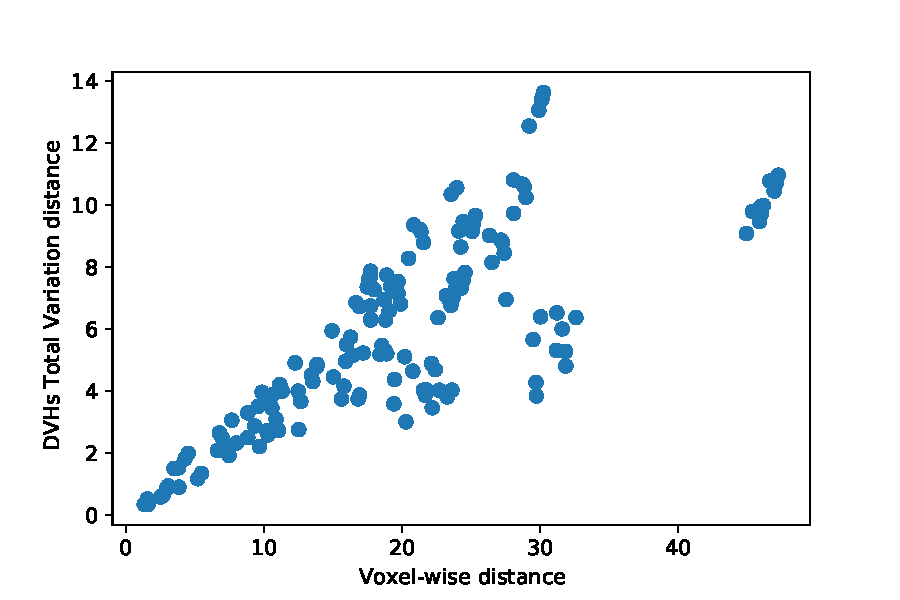
\includegraphics[width=0.49\textwidth]{dose_distances_figures/TotalVariation-Voxelwise.pdf}		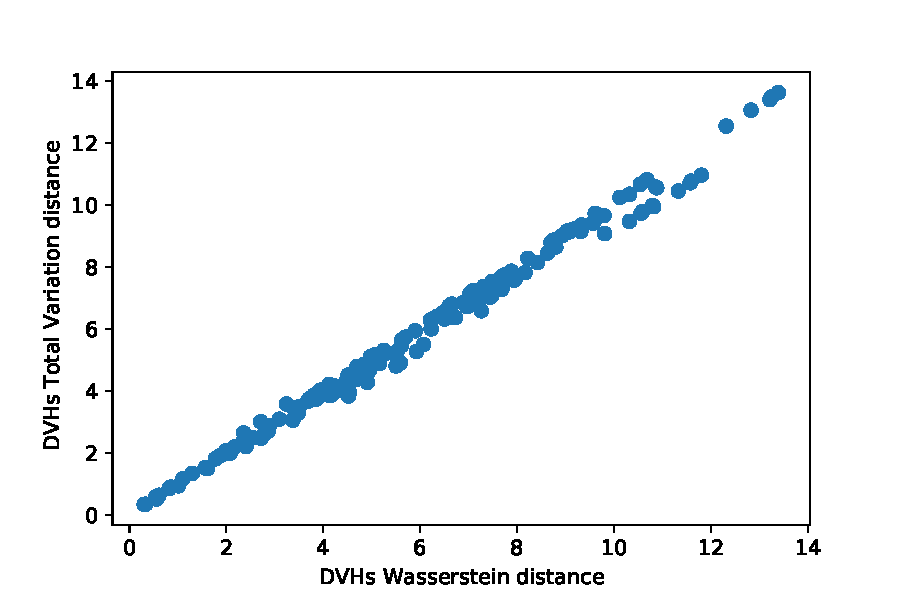
\includegraphics[width=0.49\textwidth]{dose_distances_figures/TotalVariation-Wasserstein.pdf}
	\subfloat[\label{fig:TotalVariation-Voxelwise} DVHs Total Variation vs Voxel-wise]{\hspace{.5\linewidth}}
	\subfloat[\label{fig:TotalVariation-Wasserstein} Total Variation vs Wasserstein]{\hspace{.5\linewidth}}
	\caption{Comparing Distances}
\end{figure}

\paragraph{Comparing Total Variation and Voxel-wise}
The bounding of the total variation DVH distance in terms of voxel-wise distance is clearly illustrated in Figure \ref{fig:TotalVariation-Voxelwise}, where a linear upper bound can be observed in the scatter plot.
However, specific pairs of doses are closer regarding DVH distance than initially anticipated based solely on voxel-wise comparisons.
This observation underscores the need for a more nuanced analysis beyond voxel-wise comparison, as it may overlook clinically relevant similarities between dose distributions.

\paragraph{Comparing Total Variation and Wasserstein}
Figure \ref{fig:TotalVariation-Wasserstein} shows that the two DVH distances are nearly perfectly proportional.
This result aligns with expectations, given that they are mathematically equivalent.
The only difference lies in the integration axis in the total variation distance, which accounts for the small fluctuations observed, likely due to accumulated numerical error.

\subsection{Discussion}
In this section, we introduce a novel metric for comparing radiation doses.
This metric offers the advantage of being insensitive to dose changes in certain regions, provided they are compensated in other regions, thus achieving the intended objective.
This property makes the metric particularly useful in various applications, including dose mimicking and determining early stopping criteria for fluence map optimization.

Despite the advantages, this distance metric has certain limitations.
A notable drawback is its inability to capture spatial dose distribution, which may pose challenges in specific cases.
Pathological examples exist where two DVHs appear similar, but the clinical interpretation differs significantly.
Other factors, such as the spatial distribution of the dose within the target volume or surrounding tissues, can play a pivotal role in the treatment’s effectiveness. 

For instance, two dose distributions might deliver the same high dose, with one distributed across several small regions and the other concentrated in a single large region.
While the DVHs may appear identical, clinicians would interpret these two dose distributions differently.
Such edge cases, however, are sporadic in clinical practice.
Nonetheless, for critical cases, we recommend complementing this metric with voxel-invariant approaches and other techniques to evaluate the radiation doses comprehensively.

When comparing two distinct doses, a considerable distance between them may indicate a significant difference in the intensity or frequency of the treatment.
However, this does not necessarily imply that one dose is superior.
The effectiveness of a dose depends on several other factors, such as the individual patient’s characteristics, medical history, and treatment response. 

Therefore, relying solely on the distance between doses may not accurately assess which dose is more effective or clinically appropriate in a specific case.
It is essential to account for all relevant factors when evaluating the efficacy of a treatment dose to ensure a comprehensive understanding.

Overall, the proposed dose comparison technique presents a promising tool for radiation dose evaluation.
While it has certain limitations, it can serve as a valuable addition to the repertoire of methods employed by radiation oncologists and medical physicists for optimizing treatment plans and improving patient outcomes.
Complementing existing techniques offers an additional layer of analysis, contributing to more informed decision-making in clinical practice.

\paragraph{Stop Criterion}
Defining an adequate stopping criterion for the fluence map optimization process is a critical challenge in radiotherapy dose optimization.
In clinical practice, dosimetrists often guide optimization, who may terminate the process when they are satisfied with the outcome.
However, the need for fully automated optimization processes requires the establishment of systematic and objective stopping criteria.
One potential approach is to compare the clinical effects of two dose distributions and stop when one optimization step does not change the clinical effect.
This method can helps evaluate different solutions and determine the optimal point to terminate the optimization process.



%%%%%%%%%%%%%%%%%%%%%%%%%%%%%%%%%%%%%%%%%%%%%%%%%%%%%%%%%%%%%%%%%%%%%%%%
%                                                                      %
%   %%%%%%%%%%%%%%%%%%%%%%%%%%%%%%%%%%%%%%%%%%%%%%%%%%%%%%%%%%%%%%%%   %
%   %%%%%%%%%%%%%%%%%%%%%%%%%%%%%%%%%%%%%%%%%%%%%%%%%%%%%%%%%%%%%%%%   %
%   %%%%%%%%%%%%%%%%%%%%%%%%%%%%%%%%%%%%%%%%%%%%%%%%%%%%%%%%%%%%%%%%   %
%   %%%%%%%%%%%%%%%%%%%%%%%%%%%%%%%%%%%%%%%%%%%%%%%%%%%%%%%%%%%%%%%%   %
%                                                                      %
%%%%%%%%%%%%%%%%%%%%%%%%%%%%%%%%%%%%%%%%%%%%%%%%%%%%%%%%%%%%%%%%%%%%%%%%



\section{Network of Doses}
In this section, we aim to construct a clinically meaningful network of dose distributions, where each node represents a distinct dose distribution, and the edges quantify the relationships between them.
By creating such a network, we can identify clusters of similar dose distributions and uncover patterns that reflect clinical relevance.
This network-based approach will enable us to visualize better, analyze, and interpret the relationships between various treatment plans, ultimately improving the comparison and optimization of radiotherapy strategies.

Numerous efforts have been made to automate the treatment optimization process in radiation therapy.
One promising avenue is the exploration of the Pareto frontier, as discussed in \cite{Kuipers2023} and \cite{Ottosson_2010}, which seeks to identify a set of treatment plans that balance conflicting objectives, such as maximizing tumor control while minimizing damage to surrounding healthy tissue.
Another approach proposed \cite{CristianCotrutz_2003} consists of directly extracting leaf movements from patient data to enhance the automation of dose delivery.

Despite these advancements, fully automated approaches have yet to be widely adopted in clinical practice, primarily due to practical limitations and the complexity of translating these methods into routine use.
Using doses network analysis, we will propose a hybrid approach that integrates both manual and automated treatment optimization.
This method will combine the computational efficiency of automation with the expert judgment of clinicians, ensuring that the final treatment plans are both optimal and clinically relevant.

\subsection{Methods}

\paragraph{Multiple Plans Generation}
We employed the same dose optimization process as previously described.
The cost function utilized in this study is designed to be convex, ensuring that, irrespective of the specific weight assignments given to the objectives, minimizing this cost function will consistently converge to an optimal radiotherapy plan.
To generate a diverse set of treatment doses for a given patient case and set of constraints, we optimized the cost function with varying weight assignments for each constraint.

This approach mirrors the current practice in which dosimetrists adjust the weights associated with different dose objectives to guide the optimization engine toward a clinically acceptable solution.
By altering these weights, it becomes possible to explore different trade-offs and prioritize certain aspects of the treatment plan, such as sparing healthy tissue or enhancing tumor coverage, according to the patient's specific clinical needs.

\subparagraph{Objectives’ Weights Generation}
The weights assigned to each optimization objective ($w$) dictate the relative importance of each objective in the trade-offs made by the optimization engine.
Initially, we begin with a typical weight assignment used in clinical practice.
To generate a diverse set of weights, we perturb these initial values by adding random normal noise, resulting in a unique new set of weights.

By repeating this process, we can explore a wide range of potential treatment plans.
This thorough exploration provides a nuanced understanding of the trade-offs between competing clinical objectives.
The random computational exploration of irradiation strategies extends beyond the capabilities of manual exploration, enabling clinicians to make more informed and tailored decisions based on a broader array of treatment possibilities.

\subparagraph{Dose Normalization}
For consistency across cases, we normalized the doses using the "$D_{50}$" normalization method, a common practice in radiation therapy.
This method normalizes the dose such that the median dose delivered to the PTV equals the prescribed dose, ensuring comparability across treatment plans.

\subparagraph{Phantom Patient}
Our proposed method for clustering radiation doses was evaluated using the TG-119 Prostate case \cite{AAPM-TG119}, a well-established benchmark dataset commonly employed to assess the quality of radiation therapy plans.
The TG-119 dataset provides predefined dose objectives, which were incorporated into the formulation of our cost function.
This benchmark allows for a robust evaluation of our clustering approach in the context of clinically relevant treatment goals, ensuring that the method aligns with widely accepted standards in radiation therapy planning.

\paragraph{Dose Clustering Techniques}
\subparagraph{Dose Distance}
We first needed to establish a method for defining the distance between individual doses to perform the dose clustering.
We employed the Euclidean distance between voxel-wise dose distributions as our distance metric.
The weight of each edge between two doses was then defined as the inverse of this distance as we sought to maximize the edge weights between similar doses.
Defining edge weights as the inverse of the distance between nodes is a common practice in graph theory, as noted in previous works \cite{Maleika2020} \cite{Li2018}.

\subparagraph{Community Detection}
\label{clustering_evaluation}
We employed Louvain's method for community detection to cluster the radiation doses.
Louvain's method is a greedy optimization algorithm that aims to maximize the modularity of the graph.
Modularity is a metric used to assess the quality of a graph partition by quantifying how well the graph is divided into distinct communities.
For our analysis, we utilized the implementation of Louvain's method available in the Python library NetworkX \cite{NetworkX}, which facilitated partitioning the dose similarity graph into meaningful clusters.

\paragraph{Evaluating Communities Split}
The clustering quality was evaluated using dose-volume histograms (DVHs) derived from the different doses.
We computed the mean and standard deviation of the DVH curves for each cluster and the entire dataset.

We analyzed the relative volume doses across four distinct anatomical structures.
One hundred one dose values were sampled for each structure, corresponding to volume percentages ranging from $0\%$ to $100\%$ in equal $1\%$ intervals.
These values were aggregated into a single vector, resulting in a vector of length 404 for each dose.

To assess the variability within these dose vectors, we calculated the standard deviation for each of the 404 elements in the vector.
This measure provides insight into the dispersion of dose values within the structures.
By averaging the calculated standard deviations, we derived a scalar metric that quantifies the degree of separation among the clustered doses, reflecting the consistency or variability of the doses within each group.

\subsection{Results}
\subsubsection{Doses Network}
\paragraph{Graph Plots}
%In figure \ref{fig:graph}, each node represents a dose.
%The communities are attributed using Louvain method and are identified by colors.
%Since the graph is clearly not planar, we choose to plot it in a circular layout (fig. \ref{fig:graph-circular}) and in a spring layout (fig. \ref{fig:graph-spring}).
%\begin{figure}
%	\centering
%	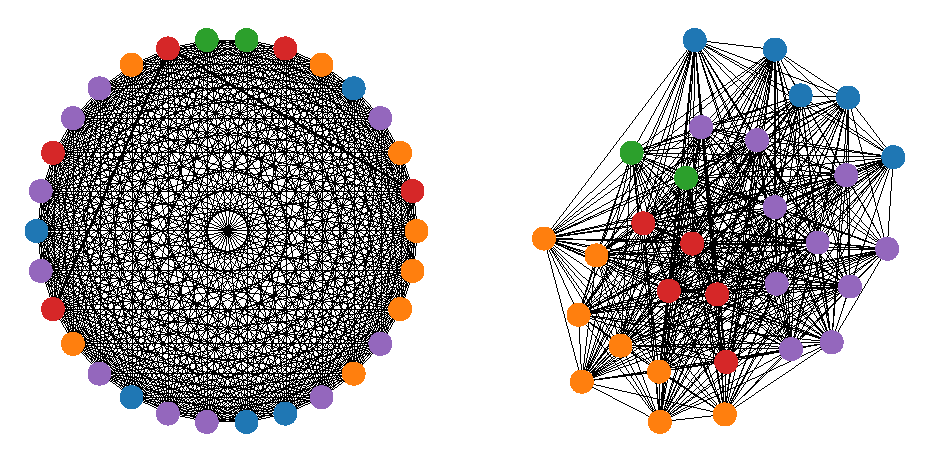
\includegraphics[width=0.40\textwidth]{dose_clustering_figures/graph.pdf}
%	\includegraphics[width=0.59\textwidth]{dose_clustering_figures/graph_bis.pdf}
%	\subfloat[\label{fig:graph-circular} (Circular Layout)]{\hspace{.5\linewidth}}
%	\subfloat[\label{fig:graph-spring} (Spring Layout)]{\hspace{.5\linewidth}}
%	\caption{
%		Plot of the Network\\
%		edges width $\propto$ edge weight $\propto$ $\nicefrac{\text{1}}{\text{distance}}$\\
%		node's color reflects community attribution
%	}
%	\label{fig:graph}
%\end{figure}

%In order to obtain a more precise understanding of the edge weights in the network, one can refer to the adjacency matrix of the edge weights, as depicted in Figure \ref{fig:adjacency}.
%\begin{figure}
%	\centering
%	\includegraphics[width=0.65\textwidth]{dose_clustering_figures/weight_adjacency_matrix.pdf}
%	\caption{Weight Adjacency Matrix of the Network}
%	\label{fig:adjacency}
%\end{figure}

\paragraph{DVH Plot}
%Figure \ref{fig:dvh} illustrates the Dose-Volume Histograms (DVHs), with the colors of the plots corresponding to the communities identified in the network analysis.
%To ensure clarity and prevent confusion, each structure is presented on a separate plot.
%Notably, our observations align with expectations, as doses assigned to nodes within the same community (indicated by the same color) exhibit nearly overlapping DVHs.
%\begin{figure}
%	\centering
%	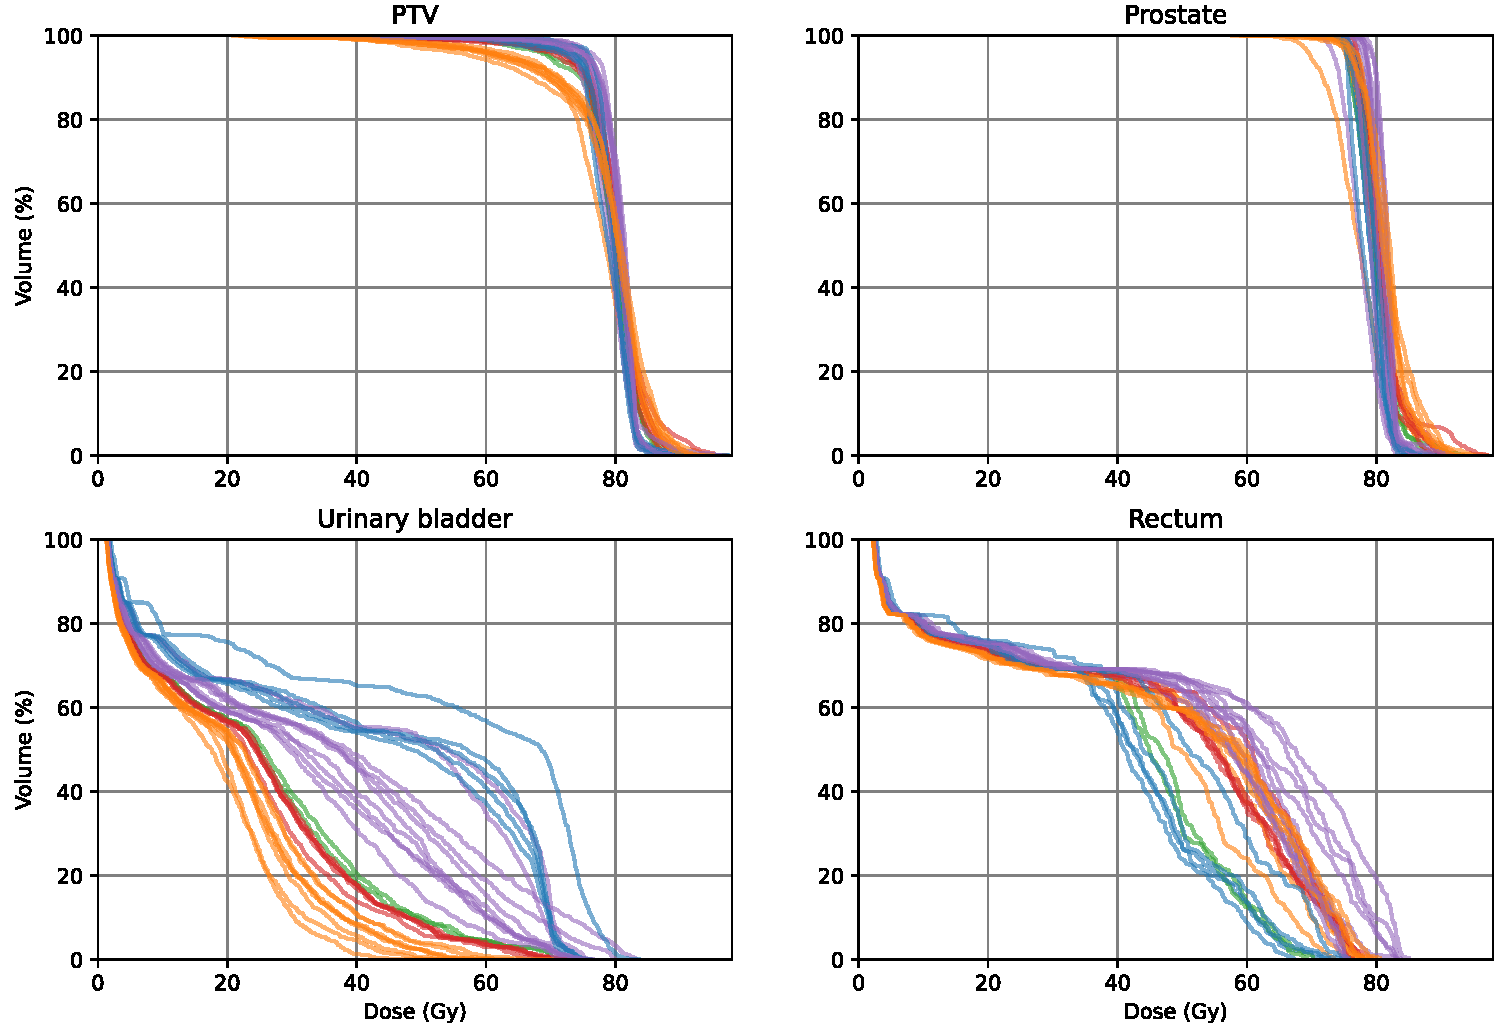
\includegraphics[width=\textwidth]{dose_clustering_figures/dvh.pdf}
%	\caption{Dose-Volume Histogram}
%	\label{fig:dvh}
%\end{figure}

%The visualization of DVHs provides valuable insights into the distribution of doses received by different structures.
%The close correspondence between dose patterns and community assignment underscores the potential of network analysis in uncovering meaningful patterns within radiation therapy data.
%By associating the colors of the DVH plots with the communities identified in the network, we gain a deeper understanding of the relationship between dose assignments and structural characteristics.
%This analysis further supports the notion that nodes (doses) within the same community share similar profiles, suggesting they could be merged, as they will likely have the same clinical effect.

\subsubsection{Dose Clustering Evaluation}
%As explained in \ref{clustering_evaluation}, we use the mean standard deviation of doses at 101 equispaced values of volume to obtain a scalar value of how far apart are a set of doses; see table \ref{table:cluster_std} for results.
%
%\begin{table}
%	\centering
%	\begin{tabular}{|l|c|c|}
%		\hline
%		Set & Set Size & Mean Standard Deviation \\
%		\hline
%		Cluster 1 \textcolor{plt-blue}  {\textbf{(blue)}}   & 4 & 2.0542 \\
%		Cluster 2 \textcolor{plt-orange}{\textbf{(orange)}} & 5 & 0.4049 \\
%		Cluster 3 \textcolor{plt-green} {\textbf{(green)}}  & 2 & 0.3618 \\
%		Cluster 4 \textcolor{plt-red}   {\textbf{(red)}}    & 2 & 0.4218 \\
%		Cluster 5 \textcolor{plt-purple}{\textbf{(purple)}} & 3 & 0.9702 \\
%		Cluster 6 \textcolor{plt-brown} {\textbf{(brown)}}  & 3 & 1.2418 \\
%		\textit{All} & \textit{19} & \textit{3.5122} \\
%		\hline
%	\end{tabular}
%	\caption{Clustering Quality}
%	\label{table:cluster_std}
%\end{table}
%
%The mean standard deviation of the clusters, with values of 2.0542, 0.4049, 0.3618, 0.4218, 0.9702, and 1.2418, averaging at 0.9091, is significantly lower (nearly 4 times lower) compared to the mean standard deviation of the full network, which is 3.5122 (see table \ref{table:cluster_std}).
%This notable reduction in standard deviation yells quantitatively that our clustering approach has favorable results.
%This quantitative assessment is further supported by qualitative results, as illustrated in Figure \ref{fig:dvh}, which demonstrates the meaningfulness and relevance of the dose clusters in characterizing radiation dose distributions.
%Our proposed clustering approach demonstrates strong performance in both qualitative and quantitative evaluations.

\subsection{Discussion}
%The ability to regroup doses into communities provides a valuable insights to understand clinical practices.
%An additional potential application of this technique is the utilization of dose clusters as a similarity measure for early stopping optimization purposes.
%Specifically, if the dose distribution exhibits similarities to the previous $n$ doses, it may serve as an indicator to halt the ongoing optimization process.
%
%However, the clustering of doses is a challenging task, as the dose space is high dimensional and the dose distribution is not smooth.
%The results presented here can not yet be used in clinical practice, they are promising and should be further investigated.

\subsection{Conclusion}
%In conclusion, this study has introduced a novel approach for clustering doses into communities based on their dose distributions, demonstrating the meaningfulness of such clustering both quantitatively and qualitatively.
%This suggests that doses belonging to the same cluster are likely to have indistinguishable clinical effects.
%
%The proposed clustering technique holds several potential applications.
%Firstly, it can be integrated into Fluence Map Optimization (FMO) to facilitate early stopping of the optimization process when the last few updates remain within the same cluster, providing efficiency gains.
%Secondly, if extended to clustering doses from different patients, it could enable the analysis of clinical center practices, offering insights into variations in treatment outcomes among centers for specific anatomies.
%
%Furthermore, this clustering approach has the potential to streamline the validation process between dosimetrists and physicists.
%Currently, multiple treatment plans are submitted for validation, leading to a cumbersome selection process for the physicist.
%However, by clustering the optimized doses with different weight parameters for constraints, the number of options can be reduced, resulting in a more efficient decision-making process and potentially reducing the personnel required in the dosimetry department.
%
%As further research and validation efforts are undertaken, this innovative approach holds considerable promise for enhancing treatment planning processes and, ultimately, improving patient outcomes.



%%%%%%%%%%%%%%%%%%%%%%%%%%%%%%%%%%%%%%%%%%%%%%%%%%%%%%%%%%%%%%%%%%%%%%%%
%                                                                      %
%   %%%%%%%%%%%%%%%%%%%%%%%%%%%%%%%%%%%%%%%%%%%%%%%%%%%%%%%%%%%%%%%%   %
%   %%%%%%%%%%%%%%%%%%%%%%%%%%%%%%%%%%%%%%%%%%%%%%%%%%%%%%%%%%%%%%%%   %
%   %%%%%%%%%%%%%%%%%%%%%%%%%%%%%%%%%%%%%%%%%%%%%%%%%%%%%%%%%%%%%%%%   %
%   %%%%%%%%%%%%%%%%%%%%%%%%%%%%%%%%%%%%%%%%%%%%%%%%%%%%%%%%%%%%%%%%   %
%                                                                      %
%%%%%%%%%%%%%%%%%%%%%%%%%%%%%%%%%%%%%%%%%%%%%%%%%%%%%%%%%%%%%%%%%%%%%%%%


\section[Novel Dosimetry Automation Approach with Graph Theory]{A Novel Framework for Multi-Objective Optimization and Robust Plan Selection Using Graph Theory (ESTRO 2024)}
% many-clicks to few-clicks solution, but goal is one-click
% N-clicks to 2/3-clicks solution, but goal is 1-click

% Poster:
% https://github.com/pauldubois98/ESTRO2024/blob/main/poster-dose_clustering.pdf
% Abstract:
% https://docs.google.com/document/d/1c5GWgAm6TgaTgsQqJVnz9GaSjIlCgfAideT8Rsz4frM/edit?usp=sharing
